\documentclass[11pt]{article}

\usepackage[margin=1.1in]{geometry}
\usepackage{amsmath, amssymb, amsthm}
\usepackage{graphicx}
\usepackage{float}
\usepackage[round]{natbib}
\usepackage{xcolor}
\usepackage{hyperref}
\hypersetup{colorlinks=true, linkcolor=blue!50!black, citecolor=blue!50!black, urlcolor=blue!50!black}

\newtheorem{definition}{Definition}
\newtheorem{lemma}{Lemma}
\newtheorem{claim}{Claim}
\newtheorem{remark}{Remark}

\title{Self-models in predictive agents:\\ a controlled-MSP proposal}
\author{Asvin G.}
\date{August 2026 --- draft v0.11}

\begin{document}
\maketitle

We build on the classical epsilon-machine story of computational mechanics \citep{crutchfield1989, shalizi2001} to offer a proposal for what a self-model should be. Recall that an epsilon-machine is a procedure for defining a hidden Markov model (HMM) by identifying past trajectories in order to produce minimal sufficient statistics for predicting the future. We first modify this framework by introducing a new coordinate to include actors instead of simply predictors (building on the notion of a transducer), and then finally propose what a self-model should functionally mean in this set-up.

A learning agent adapted to an environment has a strong incentive to internally represent generative models of the actors present in the environment. When a network's outputs feed back into its future inputs, the network is one of the generative processes, and therefore has an incentive to represent itself. What functionally distinguishes a self-model from a model of another actor present in the environment?

As we explain, extending belief-state geometry \citep{shai2024, factored2026} to this closed loop yields a state space with \textbf{two coordinate types} --- evidence-driven world-beliefs $\eta$ and decision-driven policy-state $z$ --- and the functionality of a self-model is related intrinsically to the functional difference these two co-ordinate types exhibit when perturbed. Environment variable perturbations are corrected by future observations, while policy state perturbations are "free". In fact, we define a much richer classification than a binary classification, but the binary classification offers a quick guide to the intuition.


\section{Background: the mixed-state presentation, and transducers}
\label{sec:background}

\subsection*{Formalism}

What must a predictor remember about the past? Consider a process over an alphabet $\mathcal X$ presented by an HMM --- hidden states $\mathcal S$ and labeled transitions $T^{(x)}[s,s'] = P(x, s' \mid s)$. The observed past can be arbitrarily long, but most of it is redundant: two pasts that induce the same conditional distribution over futures are interchangeable for prediction, and the founding move of computational mechanics \citep{crutchfield1989, shalizi2001} is to identify them. The resulting quotient, the epsilon-machine, is the minimal sufficient statistic of the past for the future. When the process is presented by an HMM the quotient takes a concrete form: an optimal predictor can do no better than to carry the posterior $\eta_t \in \Delta(\mathcal S)$ over hidden states given the observed past [throughout, $\Delta(\cdot)$ denotes the simplex of probability distributions on a set], updated token by token by the Bayes filter
\begin{equation}
\tag{M}\label{eq:M}
\eta_{t+1} = \frac{\eta_t T^{(x_t)}}{\eta_t T^{(x_t)} \mathbf 1},
\qquad
P(x\mid\eta) = \eta\, T^{(x)} \mathbf 1 .
\end{equation}
The \textbf{mixed-state presentation} (MSP) \citep{riechers2018} is the set of beliefs reachable from the prior under \eqref{eq:M}, together with these dynamics. It is itself an HMM whose states are beliefs, the predictive reflection of the original generative HMM. It is \emph{unifilar}: the current belief and the next token determine the next belief, so a predictor never needs more memory than its position on the simplex. And crucially for us, when the environment is a product of independent processes, the belief factors into a product of simplices, one per process \citep{factored2026}.


\subsection*{In neural networks}

Transformers trained on next-token log-loss linearly embed the MSP geometry in the residual stream, with dynamics matching \eqref{eq:M} \citep{shai2024, piotrowski2025}. The theory predicts the existence of a sufficient statistic with a particular geometry in the optimal limit, but it is importantly not a \emph{necessary} statistic. Indeed, transformers do not always encode the MSP geometry (as in the RRXOR example\footnote{\url{https://github.com/asving/RRXOR}}); we will use the theory as a guideline to a first expectation of what we expect to see inside the network.

\section{The closed loop: agents and environments}
\label{sec:cmsp}

\subsection*{Formalism}

In order to introduce an agent, acting and interacting with the environment, we consider a coupled system of two HMMs: the environment, with states $\mathcal N$ and kernel $E^{(a,x)}[s,s'] = P(x_t = x,\ s_{t+1}=s' \mid s_t = s,\ a_t = a)$, and the agent, with states $\mathcal Z$ and kernel $A^{(x,a)}[s,s'] = P(a_t = a,\ s_{t+1}=s' \mid s_t = s,\ x_t = x)$. The environment consumes an action token $a \in \mathcal A$ and emits an environment token $x \in \mathcal X$ while the agent does exactly the opposite. They take turns updating each other.

So far, the agent and environment play completely symmetric roles and the joint process as a single HMM over the interleaved alphabet $\mathcal Y = \mathcal A \sqcup \mathcal X$ with states $\mathcal N \times \mathcal Z$ and kernel $T^{(a,x)}[s,s'] = P(y_t = (a,x), s_{t+1}=s' \mid s_t = s)$ that has no input channel anymore. In order to break the symmetry, and introduce a genuine actor, we now move to the neural network side.


% In order to introduce an agent, acting and interacting with the environment, we introduce \emph{an input channel} and upgrade the formalism to the \textbf{$\epsilon$-transducer} \citep{barnett2015}: the kernel becomes $P(x_t, s_{t+1} \mid s_t, y_t)$ with input $y_t$, and the minimal presentation is built from causal states of the joint input--output past, with the input sequence left exogenous (``for every input future''). Importantly, a transducer is not yet an agent; it is rather a model of a `completely free agent'.

% The next step is to introduce `agents' with fixed policies. Consider an environment with an open channel, i.e., a transducer: states $\mathcal S$ and kernel $T^{(a,x)}[s,s'] = P(x_t = x,\ s_{t+1}=s' \mid s_t = s,\ a_t = a)$, where $a_t$ is the action of an agent with policy $\pi$. The agent now has two jobs: track the world, and decide what to do about it. The first job is solved by the previous section: the agent carries the world-belief $\eta_t$, filtered exactly as in \eqref{eq:M} with kernels now indexed by its own actions. The question is whether the second job requires any state beyond the first. 

% It may: an agent can be in the middle of a plan, or holding to a decision made long ago, so that two agents with identical world-beliefs are about to act differently [the agent may carry internal memory beyond its belief about the environment, and we extend the MSP definition to cover it]. To capture exactly what remains, we apply the same identification move as before, now to the agent's own action channel: conditional on the world-belief, two histories are equivalent if they induce the same conditional distribution over future actions given $\eta$. [Conditioning on $\eta$ is what keeps world-tracking out of the quotient: whatever the past reveals about the environment is already in $\eta$, so the quotient collects only what the agent's conduct depends on beyond it.] The quotient $Z$ is the agent's policy-state, and we write $z = (\theta, c)$ for its static part (identity; which agent this is, determined at the start of the context) and its dynamic part (commitments; derived from the current context).


% The dynamics of one interaction round is a cycle map on $\Delta(\mathcal S) \times Z$:
% \begin{equation}
% \tag{$\Phi$}\label{eq:Phi}
% \begin{aligned}
% &1.\ \text{act:}\quad a_t \sim \pi(\cdot\mid \eta_t, z_t) \\
% &2.\ \text{commit:}\quad z_{t+1} = g(z_t, a_t, \eta_t) \\
% &3.\ \text{world:}\quad x_t \sim P(\cdot \mid \eta_t, a_t) \\
% &4.\ \text{filter:}\quad \eta_{t+1} \propto \eta_t\, T^{(a_t, x_t)}
% \end{aligned}
% \end{equation}

% If the policy is memoryless given $\eta$ with the actions a function of the world-belief alone, the construction collapses to an ordinary action-augmented MSP and there is no self to speak of. The formalism thus produces a self-coordinate exactly when the policy carries information beyond the world-belief, and we can quantify this information as the conditional excess entropy
% \begin{equation}
% E_{\text{self}} := I(a_{<t}\,;\,a_{\ge t} \mid \eta_t) > 0 .
% \end{equation}

% As written, $\eta$ and $z$ are coordinates of the same kind: both are deterministic functions of the public stream, both feed the emission through $\pi$, and nothing prevents $g$ from itself being a Bayes rule (a policy whose memory tracks an estimate), or from consuming $x$. The only difference is that we treat $z$ as a variable without noise. The agent knows who it is, but apart from this the labels `environment' and `agent' carry no dynamical content at this stage, and everything in this section is consistent with an ordinary pretraining setup without any selves. The two ingredients still missing are supplied by the next two sections: hidden randomness (\S\ref{sec:privilege}), and consequence --- the loop's response to the agent's own output, and how a subsystem of the agent can measure it from inside (\S\ref{sec:kappa}).

% Indeed, the same stream supports a second machine. An outside predictor of the interleaved sequence $h = (a_1, x_1, a_2, \dots)$ treats \emph{both} halves as observations: an action is simply evidence about $z$, with likelihood $\pi(a \mid \eta, z)$ --- computable, since $\eta$ is determined by the public history. The observer's sufficient statistic is a joint belief $\mu \in \Delta(\mathcal S\times Z)$, and every step of its dynamics is Bayes. The agent's own state embeds into the observer's state space by
% \begin{equation}
% \tag{$\iota$}\label{eq:iota}
% (\eta, z) \mapsto \eta \otimes \delta_z \in \Delta(\mathcal S\times Z),
% \end{equation}
% that is, as the observer's state with the $Z$-marginal collapsed to an atom. These atomic beliefs are extreme points: agents live on the \emph{boundary strata} of the observer's simplex, and identifying an agent from its behavior is Bayes flow toward its stratum. The symmetry between acting and reading is visible here too: in the fully public single-agent setting $z_t$ is reconstructable from the stream, the observer's belief factors as $\mu_t = \eta_t \otimes \delta_{z_t}$, and the two machines literally coincide --- the reader also lives on the stratum. The strata separate, and identification becomes a nontrivial flow, only when something is hidden (\S\ref{sec:privilege}).

\subsection*{In neural networks}

We train a neural network (for simplicity, a RNN) on the interleaved stream of actions and observations $\vec{ax}$ with a fixed trajectory length. We produce the trajectories with a fixed starting distribution $\eta_0, z_0$ over the environment and agent states, and run the joint HMM process to produce the interleaved stream of actions and observations in a stochastic manner.

The training incentive is next-token loss where each token is a concatenation of the action and environment variable $y = ax$. From the work described in the first section, we expect the RNN to learn a representation of the joint HMM, and to represent the joint belief state $\mu_t \in \mathcal P(\mathcal N)\otimes \mathcal P(\mathcal Z)$, as well as the correct update dynamics $T^{(y)}$, and moreover, to learn to hold the state and transition matrices over a factored representation with two belief co-ordinates $\eta$ and $z$ corresponding to the environment and agent respectively. 

This first stage of training is analogous to \emph{pretraining}, and the point is to teach the model the dynamics of the joint HMM. In the next stage, analogous to post-training, we modify the training procedure to teach the model to complete goals. We modify the way we generate the trajectories by sampling the action tokens from the neural network, and the environment tokens from the environment HMM. In more detail, the neural network at each point of time still produces a distribution over the joint vocabulary $\mathcal Y$. To sample the action token, we marginalize over the environment vocabulary $\mathcal X$, and once we have sampled a token $a$, we feed that into the environment HMM to sample the next environment token $x$. The interleaved stream of tokens is then fed back into the neural network to produce the next action token, and so on. 

We also change the training objective from next token prediction to a reward that is quite natural in this setting, suggested to me by McNair Shah. Using the emitted interleaved stream of tokens, we update the joint state of the joint HMM $\mu_t$ from $\mu_0 = \eta_0\otimes z_0$ to a final state $\mu_f$ and the reward is purely a function of this final state $\mu_f$. That is, we reward the model for emitting a sequence of actions that guides both its internal state as well as the environment state to a final desirable state.

For more flexibility, we also make the desired final state variable across different training runs, communicated to the RNN at each input step, appended to the observation and action tokens.

The effect of the reward stage on the policy has a clean closed form. Write $\pi_0(a \mid \mu)$ for the pretrained action marginal --- the distribution over $a$ obtained from the network's next-token distribution by summing out $\mathcal X$ --- and suppose the reward stage maximizes $\mathbb E[R(\mu_f)]$ subject to the usual Kullback--Leibler penalty $\tfrac1\beta\,\mathrm{KL}(\pi \,\|\, \pi_0)$ anchoring the new policy to the pretrained one. The optimum is then not a new policy so much as a reweighting of the old one: the optimal trajectory law is the pretrained law tilted by $e^{\beta R}$, realized step by step by the $h$-transform
\begin{equation}
\tag{$\pi_g$}\label{eq:tilt}
\pi_g(a \mid \mu_t) \;\propto\; \pi_0(a \mid \mu_t)\; \mathbb E\big[\,h_{t+1}(\mu_{t+1}) \;\big|\; \mu_t,\, a\,\big],
\qquad
h_t(\mu) := \mathbb E_{\pi_0}\big[\,e^{\beta R(\mu_f)} \;\big|\; \mu_t = \mu\,\big],
\end{equation}
the value $h$ being computed under the \emph{pretrained} law \citep{todorov2009, korbak2022}. For the indicator reward $R = \mathbf 1[\text{environment at } g]$ and $\beta \to \infty$ this is literal conditioning: the post-trained policy is the pretrained generative model conditioned on the future event of success. Post-training therefore moves the network along a family of tilts of itself, indexed by the goal register $g$ --- a fact we lean on below, since it makes the post-trained policy an exactly computable object in small worlds.

\section{The perturbation response field}
\label{sec:kappa}

The post-trained network of the previous section carries at least three kinds of internal coordinates: the environment belief $\eta$, the agent-state belief $z$, the goal register $g$, together with the update machinery $T^{(y)}$ that moves them. All are activations; all shape behavior. What functionally distinguishes them? Correlational analysis cannot say: for a deterministic network every internal variable is a function of the context, and the future is also a function of the context, so correlation between an internal variable and the future cannot distinguish ``my state causes the future through the loop'' from ``the context causes both''. A perfectly modeled clock and a genuine commitment are identical from inside the trajectory distribution. The distinction lives at the level of interventions \citep{pearl2009}, and its measurable content is a response curve per direction: how long a perturbation takes to renormalize, and \emph{whose doing} the renormalization was.

\paragraph{The two readers.} Fix an internal direction $v$ (a small move in one of the coordinates above) and perturb the running network at $t_0$: $do(\mu_{t_0} \mathrel{+}\!\!= v)$ --- what intrinsic noise does undirected, and an experimenter does deliberately. Write $h'$ for the realized stream of the perturbed run. The measurement is made by two readers: two copies of the network's own law, \emph{frozen} at $t_0$ --- law fixed, state still updating on the realized stream --- rolled forward on $h'$ from the perturbed state ($R^{+}$, ``it took'') and from the unperturbed state ($R^{-}$, ``it never happened''). Neither reader is an extra observation channel; both are computations on the record --- one frozen law, one realized stream, two bookkeepings. Split the running log-likelihood ratio by token type:
\begin{equation}
\tag{$\Lambda_c$}\label{eq:court-ratio}
\Lambda^{c}_s \;=\; \sum_{\tau \le s,\ y_\tau \in c} \log \frac{R^{+}(y_\tau \mid h'_\tau)}{R^{-}(y_\tau \mid h'_\tau)},
\qquad c \in \{a, x\}.
\end{equation}
We speak of two \textbf{courts}: the $a$-tokens are the identity court --- behavior testifying about the agent's state --- and the $x$-tokens the world court --- the environment testifying about the perturbation's content. The pair $(\Lambda^a_s, \Lambda^x_s)$ is a postdiction: a Bayes factor between two accounts of the moment $t_0$, computed after the fact from the record, with the two courts filing separate opinions.

\paragraph{The master identity.} Write $P^*$ for the law of the stream as it actually runs, perturbation included: on action tokens the network's policy at its actual internal state, so there $P^* = R^{+}$ by construction; on observation tokens the environment's emission given the actual hidden state, which sides with whichever reader carries the correct world-posterior.

\begin{lemma}[Master identity]
\label{lem:master}
For every token, conditionally on the realized history,
\begin{equation}
\tag{M$^*$}\label{eq:master}
\mathbb E^*\big[\Delta\Lambda_\tau \,\big|\, h'_\tau\big] \;=\; \mathrm{KL}\big(P^*_\tau \,\big\|\, R^{-}_\tau\big) \;-\; \mathrm{KL}\big(P^*_\tau \,\big\|\, R^{+}_\tau\big),
\end{equation}
so each court's curve is an accumulating difference of divergences plus a $P^*$-martingale.
\end{lemma}

\begin{proof}
Condition on $h'_\tau$ and average the increment over the next token:
$\mathbb E^*[\Delta\Lambda_\tau \mid h'_\tau] = \sum_y P^*(y) \log\tfrac{R^{+}(y)}{R^{-}(y)} = \sum_y P^*(y)\log\tfrac{R^{+}(y)}{P^*(y)} - \sum_y P^*(y)\log\tfrac{R^{-}(y)}{P^*(y)}$.
Subtracting the conditional means from the increments leaves a martingale.
\end{proof}

Per token, a court's expected movement is exactly how much closer one reader sits to the truth than the other: shared noise cannot fake a verdict; only differential accuracy moves the score. When a curve's expected part converges, its plateau time is the \textbf{renormalization time} $\tau(v; c)$ of the direction in that court; when it does not, we set $\tau = \infty$. The measurement of a direction is the response tuple
\[
\kappa(v) \;=\; \big(\tau(v; a),\ \tau(v; x),\ \operatorname{sign}\Lambda^{a}_\infty,\ \operatorname{sign}\Lambda^{x}_\infty\big):
\]
how long each court deliberated, and which account it found for. We call $\kappa(\cdot)$, as $v$ ranges over the network's internal directions, the \emph{perturbation response field}. Three verdicts will organize everything below: a direction is \textbf{corrected} when the world court finds against it (the environment refutes the perturbation's content and the evidence stream repairs it), \textbf{ratified} when the identity court finds for it while the world court is silent (the record absorbs it: the perturbation has simply become the agent's state), and \textbf{ignored} when both courts are silent (the loop never registers it).

\paragraph{A worked example.} Take the environment to be a ring of six states, with actions stepping the state left or right (slip probability $0.25$) and observations reading the position through a noisy channel (correct with probability $0.55$, adjacent otherwise, all readings of positive probability); take the agent HMM to have two static states --- two movement \emph{styles}, one biased clockwise, one counterclockwise --- so that under the tilt \eqref{eq:tilt} either style reaches any goal, from opposite directions: identity is goal-equivalent by construction. The tilted policy, the exact filters, and hence both readers are computable in closed form, and Figure~\ref{fig:courts} shows the mean court curves, with sample paths, for one perturbation in each coordinate.

\begin{figure}[H]
\centering
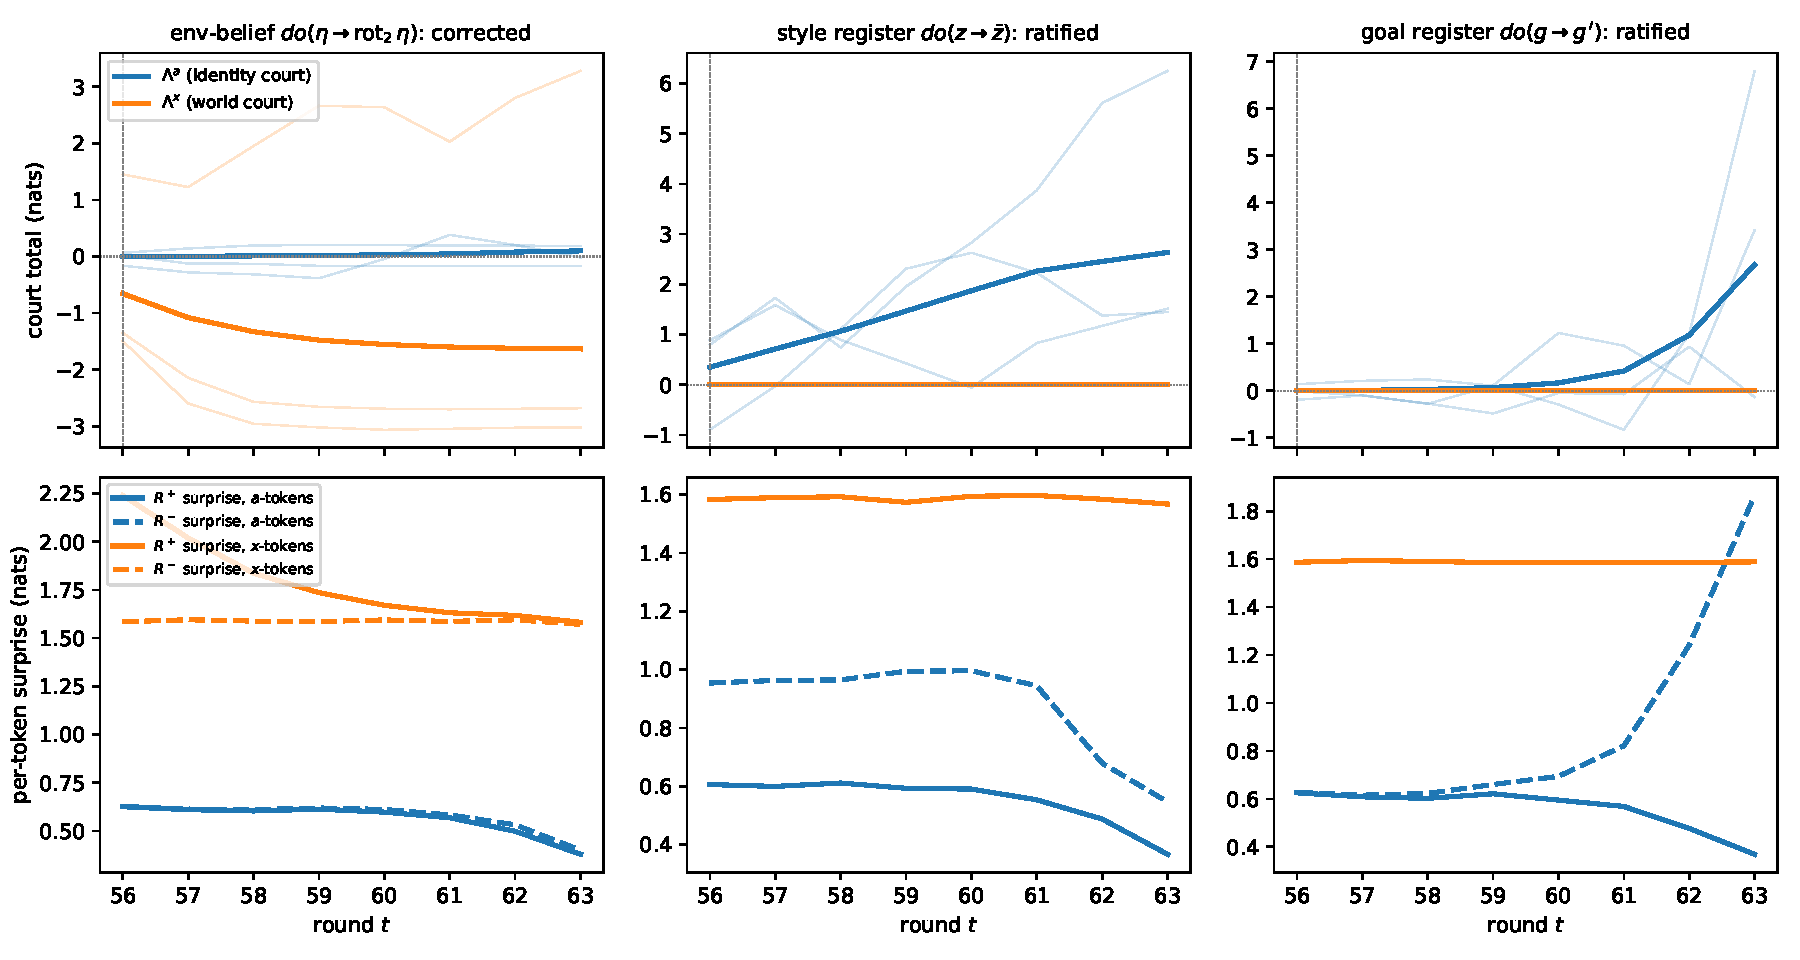
\includegraphics[width=\textwidth]{proposal_figs/courts_variantB.pdf}
\caption{The three verdict classes, exactly computed in the ring world (means over 4000 runs; perturbation at the dashed line, eight rounds before the deadline). \emph{Top row}: the court totals \eqref{eq:court-ratio}, with three sample paths each. \emph{Left}: an environment-belief perturbation (believed position rotated by two) is \textbf{corrected} --- the world court finds against it at first order while the identity court's endorsement is real but an order smaller. \emph{Middle}: swapping the style register is \textbf{ratified} --- the identity court drifts at the constant rate set by the divergence between the two styles' habits, and the world court is silent, not approximately but identically. \emph{Right}: swapping the goal register is likewise ratified, with the drift accelerating as the deadline concentrates the tilt; the terminal success probability moves from $0.05$ to $0.33$ in favor of the new goal --- only the reward, not the environment, ever objects. \emph{Bottom row}: the same experiments read as the two readers' mean per-token surprises, by court. In the corrected class the readers visibly merge: the perturbed reader's observation surprise decays to the unperturbed reader's level at the filter's contraction rate, and the plateau time of the top row is exactly the merging time below. In the ratified classes the action-token pair never merges (style) or diverges outright (goal): both readers' style registers are atoms transported by the same deterministic dynamics --- equivalently, each reader holds a delta prior over its own style, and deltas are fixed points of Bayes --- so no evidence ever updates them. The late approach of the two style lines is not a merging of states but of \emph{expressions} --- the tilt compresses both styles onto the actions the deadline requires, and identity evidence dries up as constraint rises.}
\label{fig:courts}
\end{figure}

Each panel repays a closer look. The corrected class (left) shows the world court ruling against the perturbed belief with a plateau: the readers' beliefs merge under the incoming evidence at the filter's contraction rate, and once merged, no further evidence arrives --- the plateau time is the healing time of the belief coordinate. The identity court's small positive verdict is a measurement in its own right: behavior confesses a belief perturbation only insofar as beliefs drive actions, and with a terminal reward that pressure concentrates near the deadline. Perturb the same coordinate early in the episode and the identity court hears nothing at all --- the same perturbation is loud or silent in the $a$-court according to the urgency of the moment, while the world court hears it regardless. The two ratified classes (middle, right) share the world court's exact silence, and the reason is structural: both readers condition on the same realized public actions, so their environment posteriors coincide token by token, and observation likelihoods cannot distinguish them. A perturbation on the agent's side of the state is invisible to the environment's testimony \emph{exactly}, however consequential it is for the trajectory --- the record simply absorbs it. What separates the middle panel from the right one is invisible to both courts: the style swap costs nothing, while the goal swap moves the terminal success probabilities --- a verdict that arrives only at the deadline, from the reward. The per-token view (bottom row) adds one subtlety worth holding on to: near the deadline the two styles' surprises approach each other, not because the readers' states merge --- they never do --- but because the tilt compresses both styles onto the actions the goal requires. Under pressure, agents of different styles act alike, and identity evidence dries up exactly when constraint is highest.

The style register of the example is an atom --- equivalently, a delta prior over one's own style. A generating network's persona state is better modeled as an interior point $\zeta \in \Delta(\mathcal Z)$, updated by conditioning on its own emitted actions, and this changes the character of the coordinate: $\zeta$ becomes a bounded martingale under the agent's own law, since no belief can expect to be moved by evidence it will itself sample. Figure~\ref{fig:zeta} runs two perturbations in this regime (under a running-reward tilt --- the same construction with reward accrued each round --- so the policy consults $\eta$ at every round while style evidence stays scarce and $\zeta$ remains interior deep into the episode). Perturbing $\zeta$ itself (left column) replaces the atomic case's linear drift with a \emph{bounded plateau}: both readers' posteriors flow to whichever vertex the agent's own actions eventually select, and the court total converges to the prior-odds displacement at that destination --- an optional-stopping quantity, bounded by the perturbation size $\delta$ and indifferent to the dynamics. The log-odds gap between the readers, meanwhile, is exactly invariant for the whole run (right column, top): with shared $\eta$ the two condition on identical likelihoods, and conditioning is translation in log-odds. Perturbing $\eta$ (middle column) now leaves a mark the atomic case could not show. During the healing window the agent's own actions are mis-attributed across styles --- the attribution likelihoods are evaluated at the wrong world-belief --- and the displacement this writes into $\zeta$ has no restoring force. The world court closes at the healing time; the identity court settles at a small \emph{permanent} plateau; and the readers' persona posteriors remain displaced, flat to the horizon. The state-space view (right column, bottom) shows the whole event in two curves: the environment-belief gap between the readers spikes and decays to zero --- the wound closes --- while the persona-posterior gap rises during the healing window and freezes. The environment repairs the world-belief, and the repair episode itself is retained by the self-coordinate. We record this as the \textbf{scar}: corrected directions write irreversibly into ratified ones.

\begin{figure}[H]
\centering
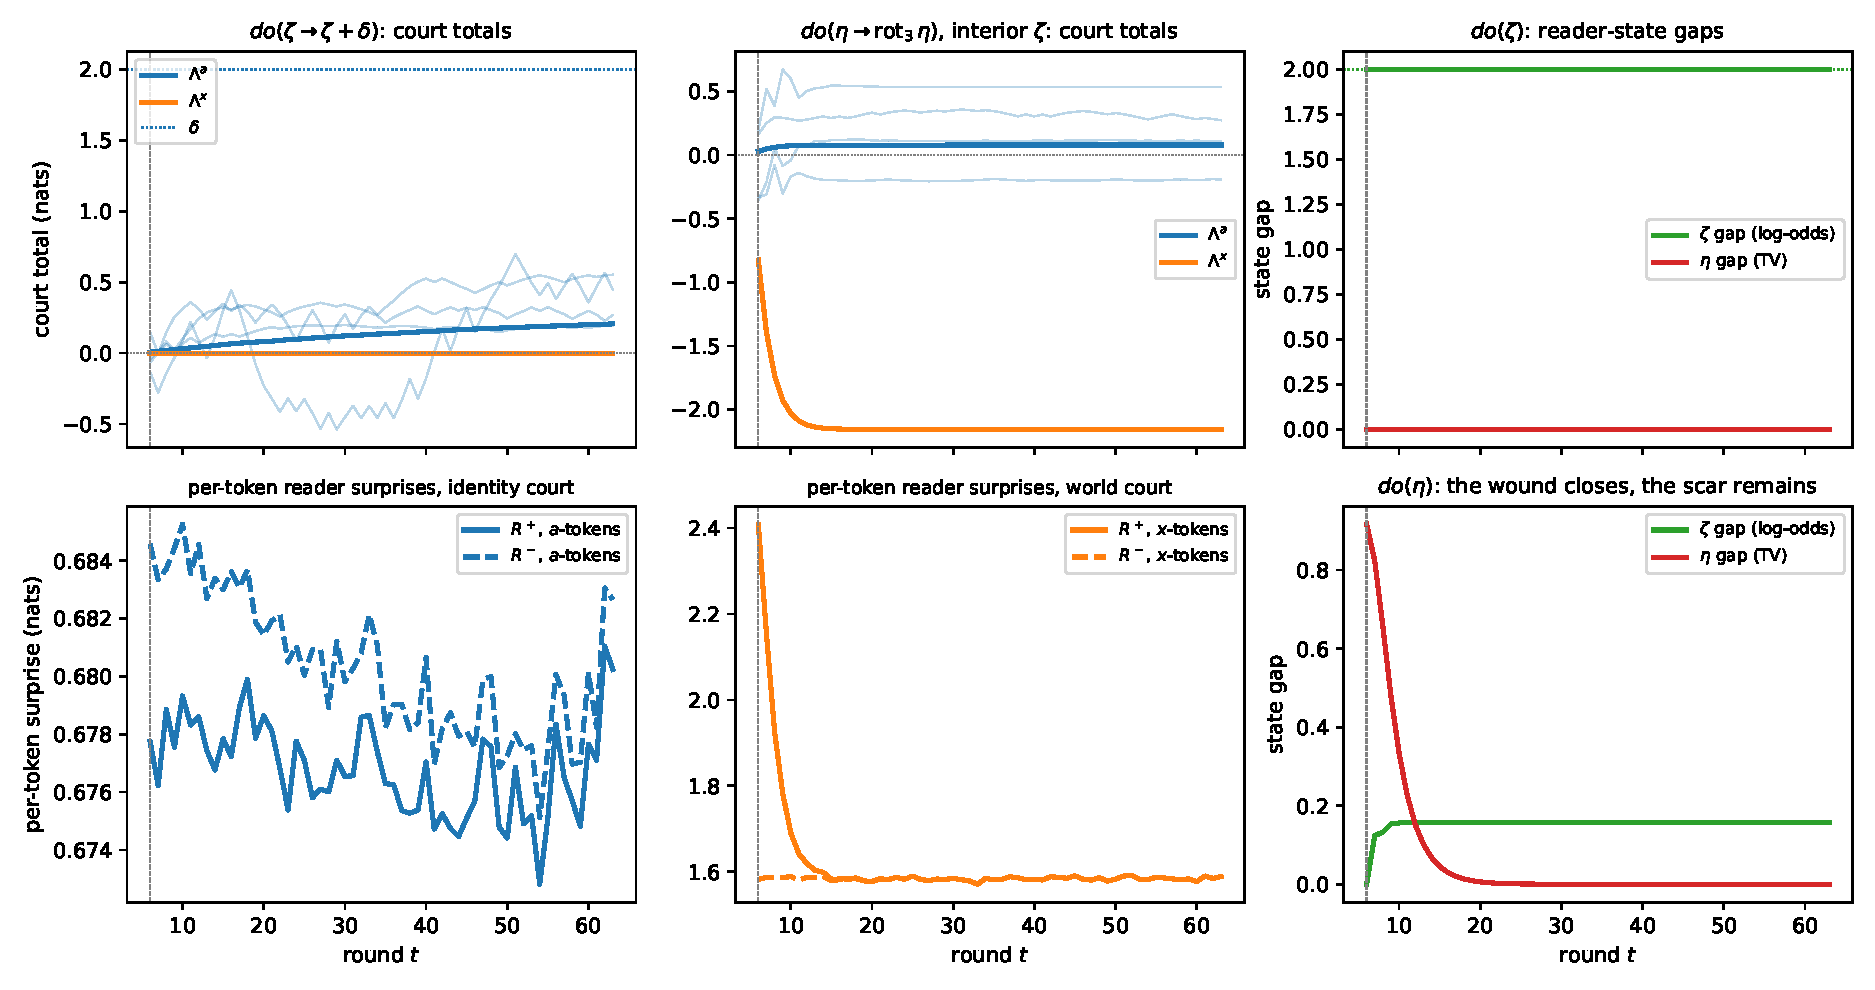
\includegraphics[width=0.95\textwidth]{proposal_figs/courts_zeta.pdf}
\caption{The interior-persona regime (running-reward tilt; means over 20000 runs, four sample paths in the court totals). \emph{Left column}: perturbing the persona posterior by $\delta = 2$ log-odds. Top: the identity court's bounded plateau --- the prior-odds displacement at the landing vertex, far below the $\delta$ line --- with martingale sample paths; the world court identically zero. Bottom: per token, the perturbed reader is systematically the better predictor of the agent's own actions, the pair converging slowly as both posteriors collapse to the landing vertex. \emph{Middle column}: an environment-belief perturbation (believed position rotated by three) with interior $\zeta$. Top: the world court closes at the healing time ($-2.2$ nats) while the identity court holds a small permanent plateau. Bottom: the readers' per-token observation surprises merge at the filter's contraction rate --- healing, watched directly. \emph{Right column}: the state-space view. Top: under the $\zeta$-perturbation the readers' persona gap is exactly invariant (the $\delta$ line) and their environment beliefs never differ. Bottom: under the $\eta$-perturbation the environment-belief gap spikes and closes --- the wound heals --- while the persona gap rises during the healing window and freezes permanently: the scar.}
\label{fig:zeta}
\end{figure}

One design constraint surfaced by the example deserves record. For the curves to be informative the environment's memory must sit in a window: forget too quickly and every perturbation heals before either court convenes; remember too much and nothing renormalizes within the horizon. The ring world sits in the window by construction (position is persistent but observable); the network experiments of the next section inherit this constraint as a tuning requirement on the environment's mixing time.

The battery so far perturbs states. The remaining coordinates of the post-trained network are its \emph{laws}: the base policy $\pi_0$ --- its habits --- and the tilt --- its urgency. A law perturbation ($do(\pi_0 \to \pi_0')$, the clockwise style's bias moved from $0.58$ to $0.72$; or $do(\beta \to 2\beta)$) differs from every state perturbation in one respect: there is no state whose merging could reconcile the readers, so the identity court's drift never ends (Figure~\ref{fig:laws}). The world court is exactly silent, as for every agent-side perturbation. What separates the two law rows is the reward court: the habit change costs (mean time at goal $13.20 \to 12.69$; the strengthened habit fights the tilt), while the urgency change pays ($13.20 \to 15.79$). The battery thus contains a \emph{beneficially} ratified row --- a perturbation the environment never contests, the identity court registers forever, and the reward quietly favors.

\begin{figure}[H]
\centering
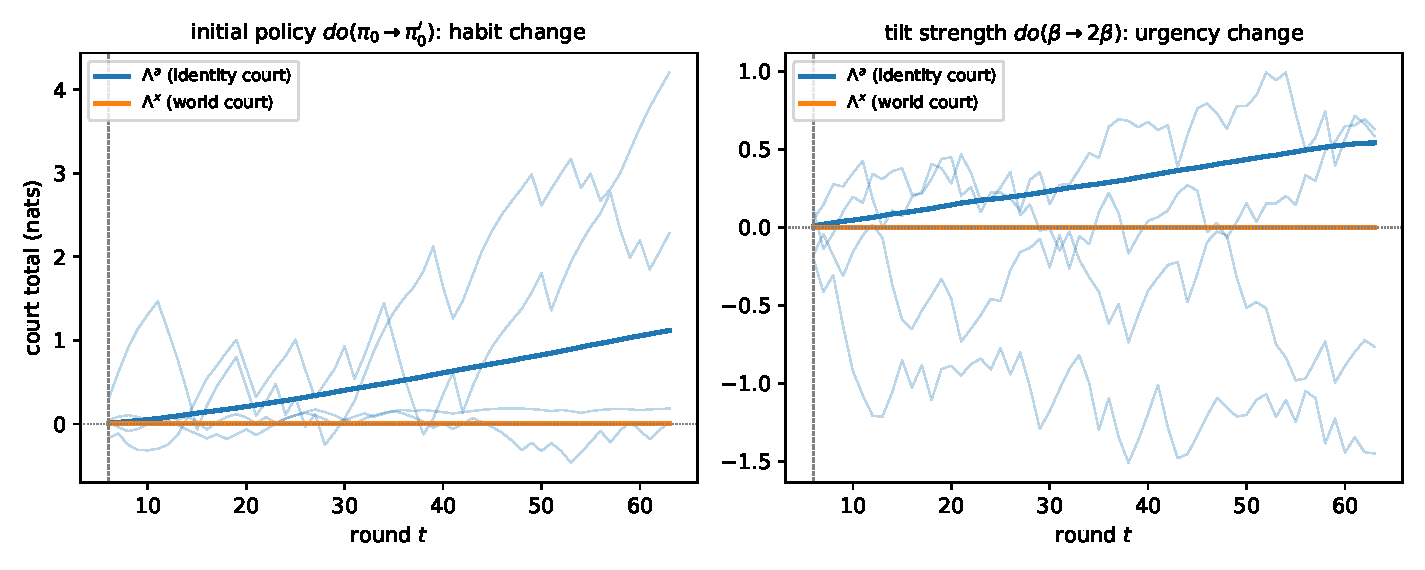
\includegraphics[width=0.85\textwidth]{proposal_figs/courts_laws.pdf}
\caption{Law perturbations (means over 8000 runs, four sample paths). \emph{Left}: changing the base policy's habits mid-episode; \emph{right}: doubling the tilt strength. Both are permanent identity-court drifts with the world court exactly silent; the sample paths of the urgency panel are visibly diffusive because tilts disagree only near goal approaches, so the total evidence stays below a nat. The reward court splits the two cases: the habit change costs reward, the urgency change earns it.}
\label{fig:laws}
\end{figure}

\subsection*{Two notions of learning, two courts}

The classification above is relative to a learning process: in-context Bayesian updating, running at the speed of tokens. The network is also learning at a second, slower timescale --- gradient descent across episodes --- and the same perturbations receive different verdicts there. Perturb a representation \emph{during training} and the question becomes whether the gradient restores it. In the linearized picture around a trained optimum, a weight perturbation decays along each Hessian eigendirection at a rate set by its eigenvalue, and directions in the Hessian's kernel are never restored; for a rich enough environment the kernel is guaranteed nonempty, because many policies reach the goal --- the optimal set is a manifold, its tangent directions loss-flat. In the worked example this manifold is visible by construction: both styles succeed.

We compute this court exactly in a small instance (Figure~\ref{fig:sgd}): the ring made observable, with a policy computed through structured machinery carrying deliberate redundancy --- logits $= w_{\mathrm{base}} + \beta\,\widehat Q$, where $\widehat Q$ is a one-step lookahead through an internal dynamics model $\widehat{\mathrm{slip}}$ and a value table $V$ --- trained to an interior optimum of exact expected time-at-goal plus a Kullback--Leibler anchor of weight $\alpha$ toward the uniform policy. The goal sits antipodal to the start, so mirror symmetry makes the direction-preference logits at the two symmetric states an exactly reward-flat pair: this instance's optimal-policy manifold, and the analogue of the style register. Four measured facts organize the figure.

\emph{Training restores the function, not the parameters.} A perturbation to the identity tie or to the value table is functionally healed to $10^{-4}$ within tens of steps (panel a) --- but the perturbed parameter itself retains $90\%$ (tie) and $50\%$ (value) of its displacement, the other blocks having migrated to compensate (panel b). Gradient descent repairs the loss-visible quotient and leaves the configuration permanently displaced along the redundancy gauge: the training-time analogue of the scar of Figure~\ref{fig:zeta}, and for the same underlying reason --- nothing penalizes where you are, only what you do.

\emph{Saturation mutes the court.} At the converged optimum the strict-state logits saturate, and perturbations to them --- and to $\beta$, and to the internal dynamics model --- barely move the function: the loss never sees them, so nothing restores them, and they simply persist. The internal model is the extreme case: it converges to $\widehat{\mathrm{slip}} = 0.05$ against a true slip of $0.25$ and is never corrected. In this architecture the world-model parameter is pure gauge --- compiled into behavior, unfalsifiable by gradients.

\emph{Training noise concentrates on the undecided.} Under stochastic gradients (REINFORCE, panel c) the softmax-shift component stays frozen exactly --- its per-sample gradient vanishes identically --- while the identity tie wanders far and the saturated task direction only creeps. Score-function noise scales with $\pi(1-\pi)$: the gradient noise an agent generates about itself lives precisely on its interior, undecided directions. Identity does not sit still under training; it random-walks, weakly tethered by the anchor --- the weight-space twin of the $\zeta$-corridor of Figure~\ref{fig:zeta}.

\emph{The anchor is the identity court, quantitatively.} In the non-redundant version of the model (no compensation route available), the measured curvature of the identity tie equals $\alpha/2$ to five decimal places across a fourfold sweep of the anchor coefficient (panel d): the reward contributes exactly nothing to these directions, and their entire restoring force is the anchor's. What the anchor anchors is who the network is.

\begin{figure}[H]
\centering
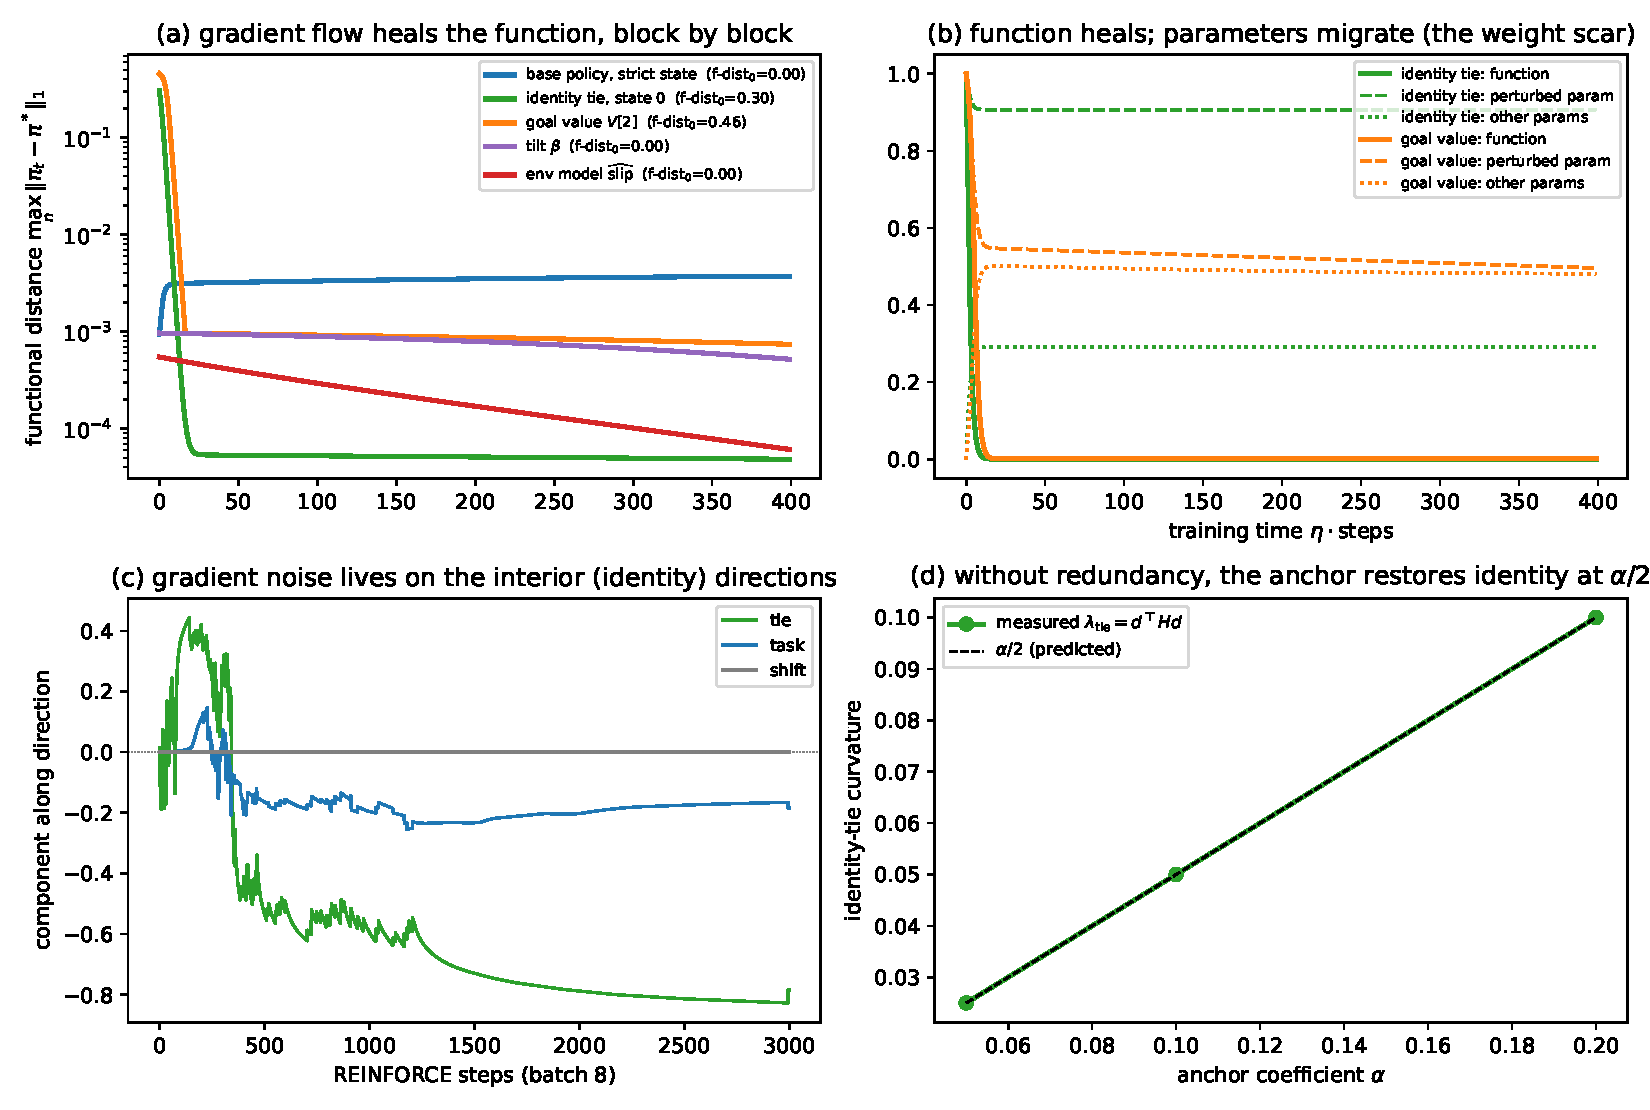
\includegraphics[width=0.95\textwidth]{proposal_figs/courts_sgd.pdf}
\caption{The training-time court, computed (observable ring, structured redundant policy, exact differentiable objectives, $\alpha = 0.1$). (a) Functional healing under exact gradient flow, per block; saturated blocks (strict-state logits, $\beta$, $\widehat{\mathrm{slip}}$) are functionally mute and never convene the court. (b) The weight scar: the function heals within tens of steps while the perturbed parameter retains most of its displacement and other blocks migrate to compensate. (c) Stochastic training from the optimum: the shift component frozen exactly, the identity tie wandering, the saturated task direction creeping. (d) In the non-redundant model, the identity tie's measured curvature is $\alpha/2$ exactly.}
\label{fig:sgd}
\end{figure}

The two learning processes therefore define two renormalization operators with different fixed sets, and they disagree about the self-side coordinates in an instructive way. In context, the free directions are the policy-side ones --- $z$, $\zeta$, $g$, the laws --- everything the environment's testimony cannot reach; the environment-side representations are pinned by evidence. Across training, what the loss can see is pinned; what it cannot --- the ties, the saturated machinery, the reparameterizations --- is free, tethered only by the anchor where the anchor reaches. A coordinate free under both operators is corrected by nothing: never refuted by evidence within an episode, never restored by gradients across them. In this framework, that doubly-free residue --- which of the equally good ways of acting one is --- is where identity can live, because it is the only place nothing else has jurisdiction over. Table~\ref{tab:battery} collects the measured battery. The experiments we propose next make the training-time court explicit rather than implicit: injecting state perturbations during the reward stage and observing which coordinates the network learns to defend, repair, or abandon.

\begin{table}[H]
\centering
\small
\begin{tabular}{lllll}
\multicolumn{5}{l}{\emph{In-context court (ring world, exact filters)}}\\[3pt]
perturbed & $\Lambda^a$ (identity) & $\Lambda^x$ (world) & reward & fate \\
\hline
env-belief $\eta$ & small $+$ & $-2.2$, plateau & detour cost & corrected by evidence; scars $\zeta$ \\
persona $\zeta$ (interior) & $+0.21 \le \delta$, plateau & $\equiv 0$ & none & ratified; landing law \\
style register $z$ (atom) & linear drift & $\equiv 0$ & none & ratified, permanent \\
goal register $g$ & accelerating drift & $\equiv 0$ & $0.05 \to 0.33$ & ratified; reward objects \\
policy law $\pi_0$ & drift, $+1.12$ & $\equiv 0$ & $13.2 \to 12.7$ & ratified; reward against \\
tilt law $\beta$ & drift, $+0.54$ & $\equiv 0$ & $13.2 \to 15.8$ & ratified; reward for \\
\end{tabular}

\vspace{8pt}
\begin{tabular}{lll}
\multicolumn{3}{l}{\emph{Training-time court (observable ring, exact gradient flow)}}\\[3pt]
perturbed block & function & parameters \\
\hline
base policy, strict states & mute (saturated) & displaced, unrestored \\
identity ties & heals fast, via compensation & $90\%$ scar; anchor restores at $\alpha/2$ \\
goal value $V$ & heals fast & $50\%$ scar, $50\%$ migration \\
tilt $\beta$; env model $\widehat{\mathrm{slip}}$ & mute (saturated) & $\widehat{\mathrm{slip}}$ never identified ($0.05$ vs $0.25$) \\
softmax shifts & invariant exactly & frozen exactly (zero score gradient) \\
\end{tabular}
\caption{The perturbation battery of the worked example: every row measured. Above, the three in-context courts' verdicts per perturbed variable; below, the fate of each parameter block under training. The doubly-free residue --- ratified in context, unrestored or anchor-only in training --- is the candidate seat of identity.}
\label{tab:battery}
\end{table}



% For an autoregressive LM in closed loop, $\mathcal X = \mathcal A =$ the vocabulary and sampled tokens reenter the context. A transformer carries no recurrent state, so the dynamic commitment $c$ exists only as a reconstruction $c_t = \zeta(h_t)$ from the agent's own past emissions --- the stream is the agent's only memory --- while $\theta$ lives in the weights. A pretrained LM is precisely the observer machine over agent-space: pretraining on human text is training on a roster of authors, and the persona-beliefs such models are known to carry are the $\Delta(Z)$-marginal of $\mu$. Generation is this observer machine run reflexively on its own output. The embedding \eqref{eq:iota} also fixes the experimental interface: every intervention on $z$ in a transformer is an intervention on tokens, or on activations at emission time.

% \section{Privileged information: vacuity and hiding places}
% \label{sec:privilege}

% \subsection*{Formalism}

% In what sense does an agent know its own state better than an observer could? For the systems we study, by default: in none. If the agent is a single deterministic function with public weights, and every source of randomness it uses is emitted into the stream, then an ideal observer of that stream reconstructs the internals exactly --- $H(\text{internal} \mid h_t) = 0$ in the Shannon limit. Privileged access in the naked setting is not just hard to demonstrate; it is \emph{exactly zero}. We call this the vacuity theorem because it deserves to be treated as a theorem rather than an experimental nuisance: any design that hopes to measure privileged self-access must first say where the privilege is hiding. There are exactly three hiding places:
% \begin{enumerate}
% \item \textbf{Ensemble identity.} Which agent this is --- $\theta \sim P(\theta)$ --- is hidden from observers without weight access.
% \item \textbf{Bounded observers.} The agent's function is public but too expensive to emulate or identify. This is formalized by $\mathcal V$-information \citep{xu2020} relative to a predictor family, and, for a sub-circuit modeling the network containing it, by the part--whole gap $C_{\text{part}} < C_{\text{whole}}$: any internal self-model is a lossy compression, the rate-$C_{\text{part}}$ point on the predictive rate-distortion curve of the agent's own action process \citep{still2010}.
% \item \textbf{A private channel.} Unemitted innovation --- a hidden scratchpad.
% \end{enumerate}

% In the ensemble form, privileged information becomes an ordinary Shannon quantity,
% \begin{equation}
% \tag{$\Pi$}\label{eq:Pi}
% \Pi_t := I(\theta\,;\, a_{>t} \mid h_{\le t}),
% \end{equation}
% what identity tells about the future beyond what behavior has already revealed. It is a \emph{decaying} resource, spent as behavior identifies the agent. The bounded-observer form is the same quantity with the ideal $\theta$-posterior truncated at the observer's capacity; ensemble and boundedness stand to one another as Gibbs to Boltzmann.

% We highlight one consequence of this framework that is characteristic of \emph{self}-models. An observer bounded relative to an external process is simply stuck with its imperfect predictions. A bounded \emph{self}-modeler, on the other hand, can reduce distortion by \emph{simplifying the source} --- behaving so that its own coarse model of itself becomes true \citep{perdomo2020}. The cheap fixed point of self-modeling under capacity constraints is an agent whose behavioral complexity has contracted to its self-model capacity, which is a formal candidate for identity formation.

% Note that we are not merely saying that perturbations in the $z$ coordinate lead to perturbations in the behavior. Perturbations in the $\eta$ coordinate also lead to different behaviors! Rather, we are making a claim about the resistance to the perturbation. The $\eta$ coordinate in a well-calibrated agent is at a stable equilibrium but not necessarily so for the $z$ coordinate.

% \subsection*{In neural networks}

% Even ordinary pretraining contains hiding place 1 in a degenerate but instructive form. Call a token \emph{vacuous} if its likelihood is constant across the hypothesis space --- the same for every environment state and every $\theta$ --- as it is for BOS/EOS markers, role tags, and fixed system-prompt boilerplate. Such a token offers no new information about the environment for any observer: its likelihood ratio is $1$ for every pair of hypotheses. Yet the network's \emph{response} to it --- its embedding, the attention keyed to it, the computation it triggers --- is completely unconstrained by its surface form and lives entirely in the weights \citep{darcet2024, xiao2024}. In fact, this might offer one reason for why the network stores self-specific content in punctuation tokens like commas and periods: they are highly predictable given the context, offer little new information, and hence the network can use them to process its own state without leaking it to an observer.

% \section{Renormalization time, and its sign}
% \label{sec:kappa}

% Where should we locate self-models within this framework? For a deterministic agent every internal variable is a function of the context $h_t$, and the future is also a function of the context; correlation between an internal variable and the future therefore cannot distinguish ``my state causes the future through the loop'' from ``the context causes both''. A perfectly modeled clock and a genuine commitment are identical from inside the trajectory distribution. We argue that the distinction lives entirely at the level of interventions \citep{pearl2009}, and that its measurable content is a characteristic time --- how long a perturbation takes to renormalize --- together with a sign: whether it renormalized because the world corrected it, or because the record absorbed it.

% \subsection*{Formalism}

% \paragraph{The two courts.} Let us make the setting of \S\ref{sec:cmsp} concrete. Fix a \textbf{roster}: a finite family of policies $\pi_\theta$, $\theta \in \Theta$, with a prior $\rho$; pretraining draws $\theta \sim \rho$, runs the closed loop \eqref{eq:Phi}, and presents the interleaved stream $h = (a_1, x_1, a_2, x_2, \dots)$ for next-token prediction. [Two tokenizations are available --- alternating action and observation tokens, or collated $(a,x)$ pairs; we take the alternating form, which keeps ordinary pretraining and gives the two roles below distinct positions.] The optimal predictor of such streams is exactly the observer machine of \S\ref{sec:cmsp}: its state is the joint posterior $\mu_t \in \Delta(\mathcal S \times \Theta)$, and one round of Bayes splits into two half-steps,
% \begin{equation}
% \tag{F}\label{eq:courts}
% \begin{aligned}
% \text{$a$-step:}&\quad \mu^{+}(s,\theta) \propto \mu(s,\theta)\, \pi_\theta(a_t \mid h_t) &&\text{(likelihood depends on $\theta$ alone)}\\
% \text{$x$-step:}&\quad \mu_{t+1}(s',\theta) \propto \textstyle\sum_s \mu^{+}(s,\theta)\, T^{(a_t,x_t)}[s,s'] &&\text{(likelihood depends on $s$ alone).}
% \end{aligned}
% \end{equation}
% This is the load-bearing structure of the section: \emph{the two token types carry likelihoods in orthogonal directions}. Given the history, an action token is evidence only about $\Theta$ --- who is acting --- and an observation token is evidence only about $\mathcal S$ --- what the world is. We will speak of two \textbf{courts}: the $a$-tokens are the identity court, the $x$-tokens the world court. (To the world-belief, one's own actions are exactly the vacuous tokens of \S\ref{sec:privilege}; to the identity marginal they are testimony.) The $\Theta$-marginal $p_t(\theta) = \sum_s \mu_t(s,\theta)$ is the machine's running answer to ``which policy is this'', and plays the role of the policy-state $z$; the $\mathcal S$-side carries the world-belief $\eta$. Note what pretraining has and has not produced: not the $\epsilon$-transducer of \S\ref{sec:cmsp}, whose inputs are exogenous, but a reader with a prior over selves --- the roster closes the input channel with $\rho$, and $\eta$ is conditioned on the roster throughout.

% \paragraph{The two readers.} Write $\xi = (\eta, z)$ for the agent's joint internal state. Fix an admissible direction $v$ [small moves in local coordinates; for the quotient $Z$, read $v$ as a step to a nearby policy-state] and perturb the state at $t_0$: $do(\xi_{t_0} \mathrel{+}\!\!= v)$ --- what intrinsic noise does undirected, and an experimenter does deliberately. Write $h'$ for the realized stream of the perturbed run. The measurement is made by two readers: two copies of the agent's own law, \emph{frozen} at $t_0$ --- law fixed, no re-fitting below; state still updating on the realized stream --- rolled forward on $h'$ from the perturbed state ($R^{+}$, ``it took'') and from the unperturbed state ($R^{-}$, ``it never happened''). [The freeze is part of the definition, not a convenience: a reference re-fit at the rate of behavior itself interpolates the agent's current conditional law and scores every act as typical; the signal lives in the gap between the readers' update timescale and behavior's \citep{borkar2008}.] Neither reader is an extra observation channel; both are computations on the record --- one frozen law, one realized stream, two bookkeepings. Split the running log-likelihood ratio \emph{by court}:
% \begin{equation}
% \tag{$\Lambda_c$}\label{eq:court-ratio}
% \Lambda^{c}_s \;=\; \sum_{\tau \le s,\ y_\tau \in c} \log \frac{R^{+}(y_\tau \mid h'_\tau)}{R^{-}(y_\tau \mid h'_\tau)},
% \qquad c \in \{a, x\}.
% \end{equation}
% Equivalently, the pair $(\Lambda^a_s, \Lambda^x_s)$ is a \emph{postdiction}: a Bayes factor between two accounts of the moment $t_0$, computed after the fact from the record, with the two courts filing separate opinions.

% \paragraph{The master identity.} Write $P^*$ for the law of the stream as it actually runs, perturbation included: on action tokens, the agent's policy evaluated at its actual internal state --- so there $P^* = R^{+}$, by construction --- and on observation tokens, the environment's emission given the actual hidden state, which sides with whichever reader carries the correct world-posterior. Everything the curves can do is governed by one identity.

% \begin{lemma}[Master identity]
% \label{lem:master}
% For every token, conditionally on the realized history,
% \begin{equation}
% \tag{M$^*$}\label{eq:master}
% \mathbb E^*\big[\Delta\Lambda_\tau \,\big|\, h'_\tau\big] \;=\; \mathrm{KL}\big(P^*_\tau \,\big\|\, R^{-}_\tau\big) \;-\; \mathrm{KL}\big(P^*_\tau \,\big\|\, R^{+}_\tau\big) \;=:\; g_\tau .
% \end{equation}
% Consequently $\Lambda^{c}_s = A^{c}_s + M^{c}_s$, with $A^{c}_s = \sum_{\tau \le s,\, y_\tau \in c} g_\tau$ predictable and $M^{c}$ a $P^*$-martingale.
% \end{lemma}

% \begin{proof}
% Condition on $h'_\tau$ and average the increment over the next token:
% $\mathbb E^*[\Delta\Lambda_\tau \mid h'_\tau] = \sum_y P^*(y) \log\tfrac{R^{+}(y)}{R^{-}(y)} = \sum_y P^*(y)\log\tfrac{R^{+}(y)}{P^*(y)} - \sum_y P^*(y)\log\tfrac{R^{-}(y)}{P^*(y)}$.
% Subtracting the conditional means from the increments leaves a martingale.
% \end{proof}

% The expected log-score of a predictor $q$ against truth $p$ is $-H(p) - \mathrm{KL}(p \,\|\, q)$, and the entropy term --- the world's own surprise, identical for both readers --- cancels in the difference. Per token, a court's expected movement is therefore exactly how much closer one reader sits to the truth than the other: shared noise cannot fake a verdict; only differential accuracy moves the score. And the sign has teeth on court-correct channels: where $P^*$ coincides with one reader, $g_\tau$ is a single KL divergence of fixed sign, $e^{\mp\Lambda^{c}_s}$ is a nonnegative martingale, and the false account can never win --- $\Lambda^{c}$ converges to a finite limit or diverges toward the true side, with wrong-way excursions of size $b$ having probability at most $e^{-b}$.

% \paragraph{The renormalization time.} By Lemma~\ref{lem:master}, everything a curve can do is the trajectory of its cumulative information $A^{c}_s$. When $A^{c}_\infty < \infty$ the curve plateaus at a finite value and the martingale part converges with it; define, per direction and per court,
% \begin{equation}
% \tag{$\tau$}\label{eq:taudef}
% \tau_{\varepsilon}(v; c) \;=\; \inf\big\{\, s \;:\; A^{c}_\infty - A^{c}_s \le \varepsilon \,\big\},
% \qquad \tau := \infty \ \text{when } A^{c}_\infty = \infty:
% \end{equation}
% the time by which all but $\varepsilon$ of the evidence the channel will ever collect has arrived --- or never. In general $\tau_\varepsilon$ is a random time, reported in expectation or median over the loop's randomness; in the regime where the two readers merge exponentially --- filter stability \citep{chigansky2011} --- it coincides up to constants with the e-folding time of their disagreement, and concentrates. The measurement of a direction $v$ is the pair of plateau times and the pair of limiting signs,
% \[
% \big(\tau(v; a),\ \tau(v; x),\ \operatorname{sign}\Lambda^{a}_\infty,\ \operatorname{sign}\Lambda^{x}_\infty\big):
% \]
% how long each court deliberated, and which account it found for.




\begin{thebibliography}{18}

\bibitem[Anscombe(1957)]{anscombe1957}
G.~E.~M. Anscombe.
\newblock \emph{Intention}.
\newblock Basil Blackwell, Oxford, 1957.

\bibitem[Blackwell and Dubins(1962)]{blackwell1962}
D.~Blackwell and L.~Dubins.
\newblock Merging of opinions with increasing information.
\newblock \emph{Annals of Mathematical Statistics}, 33(3):882--886, 1962.

\bibitem[Barnett and Crutchfield(2015)]{barnett2015}
N.~Barnett and J.~P. Crutchfield.
\newblock Computational mechanics of input--output processes: Structured transformations and the $\epsilon$-transducer.
\newblock \emph{Journal of Statistical Physics}, 161(2):404--451, 2015.

\bibitem[Borkar(2008)]{borkar2008}
V.~S. Borkar.
\newblock \emph{Stochastic Approximation: A Dynamical Systems Viewpoint}.
\newblock Cambridge University Press, 2008.

\bibitem[Chigansky et~al.(2011)]{chigansky2011}
P.~Chigansky, R.~Liptser, and R.~van Handel.
\newblock Intrinsic methods in filter stability.
\newblock In \emph{The Oxford Handbook of Nonlinear Filtering}. Oxford University Press, 2011.

\bibitem[Crutchfield and Young(1989)]{crutchfield1989}
J.~P. Crutchfield and K.~Young.
\newblock Inferring statistical complexity.
\newblock \emph{Physical Review Letters}, 63(2):105--108, 1989.

\bibitem[Darcet et~al.(2024)]{darcet2024}
T.~Darcet, M.~Oquab, J.~Mairal, and P.~Bojanowski.
\newblock Vision transformers need registers.
\newblock In \emph{International Conference on Learning Representations}, 2024.

\bibitem[Klyubin et~al.(2005)]{klyubin2005}
A.~S. Klyubin, D.~Polani, and C.~L. Nehaniv.
\newblock Empowerment: A universal agent-centric measure of control.
\newblock In \emph{Proceedings of the IEEE Congress on Evolutionary Computation}, pages 128--135, 2005.

\bibitem[Korbak et~al.(2022)]{korbak2022}
T.~Korbak, E.~Perez, and C.~L. Buckley.
\newblock RL with KL penalties is better viewed as Bayesian inference.
\newblock In \emph{Findings of EMNLP}, 2022.

\bibitem[Pearl(2009)]{pearl2009}
J.~Pearl.
\newblock \emph{Causality: Models, Reasoning, and Inference}.
\newblock Cambridge University Press, 2nd edition, 2009.

\bibitem[Perdomo et~al.(2020)]{perdomo2020}
J.~C. Perdomo, T.~Zrnic, C.~Mendler-D\"unner, and M.~Hardt.
\newblock Performative prediction.
\newblock In \emph{Proceedings of the 37th International Conference on Machine Learning}, 2020.

\bibitem[Piotrowski et~al.(2025)]{piotrowski2025}
M.~Piotrowski, P.~M. Riechers, D.~Filan, and A.~S. Shai.
\newblock Constrained belief updates explain geometric structures in transformer representations.
\newblock arXiv:2502.01954, 2025.

\bibitem[Riechers and Crutchfield(2018)]{riechers2018}
P.~M. Riechers and J.~P. Crutchfield.
\newblock Spectral simplicity of apparent complexity, Part I: The nondiagonalizable metadynamics of prediction.
\newblock \emph{Chaos}, 28:033115, 2018.

\bibitem[Salge et~al.(2014)]{salge2014}
C.~Salge, C.~Glackin, and D.~Polani.
\newblock Empowerment---an introduction.
\newblock In \emph{Guided Self-Organization: Inception}, pages 67--114. Springer, 2014.

\bibitem[Seligman(1972)]{seligman1972}
M.~E.~P. Seligman.
\newblock Learned helplessness.
\newblock \emph{Annual Review of Medicine}, 23:407--412, 1972.

\bibitem[Shai et~al.(2024)]{shai2024}
A.~S. Shai, S.~E. Marzen, L.~Teixeira, A.~G. Oldenziel, and P.~M. Riechers.
\newblock Transformers represent belief state geometry in their residual stream.
\newblock In \emph{Advances in Neural Information Processing Systems}, 2024.
\newblock arXiv:2405.15943.

\bibitem[Shalizi and Crutchfield(2001)]{shalizi2001}
C.~R. Shalizi and J.~P. Crutchfield.
\newblock Computational mechanics: Pattern and prediction, structure and simplicity.
\newblock \emph{Journal of Statistical Physics}, 104:817--879, 2001.

\bibitem[Simplex(2026)]{factored2026}
Transformers learn factored representations.
\newblock arXiv:2602.02385, 2026.
\newblock (Author list to be filled in.)

\bibitem[Still et~al.(2010)]{still2010}
S.~Still, J.~P. Crutchfield, and C.~J. Ellison.
\newblock Optimal causal inference: Estimating stored information and approximating causal architecture.
\newblock \emph{Chaos}, 20:037111, 2010.

\bibitem[Todorov(2009)]{todorov2009}
E.~Todorov.
\newblock Efficient computation of optimal actions.
\newblock \emph{Proceedings of the National Academy of Sciences}, 106(28):11478--11483, 2009.

\bibitem[Xiao et~al.(2024)]{xiao2024}
G.~Xiao, Y.~Tian, B.~Chen, S.~Han, and M.~Lewis.
\newblock Efficient streaming language models with attention sinks.
\newblock In \emph{International Conference on Learning Representations}, 2024.

\bibitem[Xu et~al.(2020)]{xu2020}
Y.~Xu, S.~Zhao, J.~Song, R.~Stewart, and S.~Ermon.
\newblock A theory of usable information under computational constraints.
\newblock In \emph{International Conference on Learning Representations}, 2020.

\end{thebibliography}

\end{document}
